\documentclass{article}

% NeurIPS 2024 style
\usepackage[final]{neurips_2024}

% Packages
\usepackage[utf8]{inputenc}
\usepackage[T1]{fontenc}
\usepackage{hyperref}
\usepackage{url}
\usepackage{booktabs}
\usepackage{amsfonts}
\usepackage{nicefrac}
\usepackage{microtype}
\usepackage{xcolor}
\usepackage{graphicx}
\usepackage{subcaption}
\usepackage{amsmath}
\usepackage{amssymb}
\usepackage{algorithm}
\usepackage{algorithmic}
\usepackage{multirow}
\usepackage{tikz}
\usepackage{pgfplots}
\usepackage{pgfplotstable}
\pgfplotsset{compat=1.17}

% Custom commands
\newcommand{\E}{\mathbb{E}}
\newcommand{\R}{\mathbb{R}}
\newcommand{\cA}{\mathcal{A}}
\newcommand{\cD}{\mathcal{D}}
\newcommand{\cI}{\mathcal{I}}
\newcommand{\cS}{\mathcal{S}}

\title{Scaling Laws for Counterfactual Value Prediction in \\
No-Limit Hold'em: MLPs vs Grouped-Token Transformers}

\author{
  Naman Bajpai \\
  Drexel University \\
  \texttt{naman.bajpai@drexel.edu}
}

\begin{document}

\maketitle

\begin{abstract}
Counterfactual value (CFV) prediction is a core primitive for learning approximate Nash equilibria in large imperfect-information games such as No-Limit Texas Hold'em (NLHE). While multilayer perceptrons (MLPs) remain the default architecture for CFV regression, Transformers have demonstrated superior scaling in structured domains---provided the representation preserves semantics while keeping attention tractable. We present a controlled scaling study comparing MLPs against a \textbf{Grouped-Token Transformer} for NLHE CFV prediction, trained on counterfactual advantage targets from Monte Carlo CFR. Our key contribution is a \textbf{semantic tokenization} of the 141-dimensional flat encoding into \textbf{24 meaningful tokens}: card bucket, round indicator, state features, and a 20-step action history. This reduces attention complexity from $O(141^2)$ to $O(24^2)$---a 34$\times$ reduction. Across data scales from 50K to 10M samples and model scales from 14K to 25M parameters, we fit power laws $L(N) \propto N^{-\alpha}$ and find the Transformer exhibits a \textbf{3.5$\times$ steeper scaling exponent}: $\alpha_{\text{Trans}} = 0.42 \pm 0.03$ vs $\alpha_{\text{MLP}} = 0.12 \pm 0.02$. At 10M samples, this translates to \textbf{3.2$\times$ lower validation MSE} (0.089 vs 0.284). These results establish Transformers with semantic tokenization as the dominant architecture for neural CFR.
\end{abstract}

%==============================================================================
\section{Introduction}
%==============================================================================

No-Limit Texas Hold'em (NLHE) is a canonical benchmark for decision-making under hidden information~\citep{bowling2015heads,brown2019superhuman}. With $\sim 10^{164}$ game states, exact solutions are intractable. Modern systems rely on abstraction and regret-minimization methods like CFR~\citep{zinkevich2007regret} paired with function approximation.

A central subproblem is learning $f_\theta: \cI \rightarrow \R^{|\cA|}$---mapping infoset encodings to counterfactual values. Prior work~\citep{moravvcik2017deepstack,brown2019superhuman} uses MLPs on dense feature vectors. However, NLHE is inherently \textbf{sequence-dependent}: betting history is ordered, public state evolves by round, and optimal responses depend on temporal context.

Transformers~\citep{vaswani2017attention} excel at sequence modeling, but naïvely treating each scalar feature as a token yields $O(141^2) \approx 20{,}000$ attention pairs per layer. The core question is:

\begin{quote}
\textit{Do Transformers exhibit superior scaling laws for CFV prediction when tokenized to match NLHE's semantic structure?}
\end{quote}

We answer \textbf{yes}. Our contributions:

\begin{enumerate}
    \item \textbf{Grouped-Token Transformer}: Semantic tokenization compressing 141 features into 24 tokens, reducing attention cost by 34$\times$ (\S\ref{sec:representation}).
    
    \item \textbf{Scaling Law Characterization}: First measurement of neural scaling laws for CFV prediction. We fit $L(N) = C \cdot N^{-\alpha}$ and find $\alpha_{\text{Trans}} = 0.42$ vs $\alpha_{\text{MLP}} = 0.12$---a 3.5$\times$ advantage (\S\ref{sec:scaling}).
    
    \item \textbf{3.2$\times$ Performance Gap}: At 10M samples, Trans-XXL achieves MSE = 0.089 vs MLP-XXL's 0.284 (\S\ref{sec:results}).
\end{enumerate}

%==============================================================================
\section{Background}
%==============================================================================

\subsection{Counterfactual Regret Minimization}

CFR~\citep{zinkevich2007regret} computes Nash equilibria by accumulating regrets. The counterfactual value for action $a$ at infoset $I$ is:
\begin{equation}
    v(I, a) = \sum_{z \in Z_I^a} \pi^{-i}(z) \cdot u_i(z)
\end{equation}

Monte Carlo CFR (MCCFR)~\citep{lanctot2009monte} samples trajectories for scalability. Deep CFR~\citep{brown2019deep} trains neural networks to predict CFVs:
\begin{equation}
    \mathcal{L}(\theta) = \E_{(x, y) \sim \cD} \left[ \| f_\theta(x) - y \|^2 \right]
\end{equation}

\subsection{Neural Scaling Laws}

\citet{kaplan2020scaling} established power-law relationships:
\begin{equation}
    L(N) = \left(\frac{N_c}{N}\right)^{\alpha_N}, \quad L(D) = \left(\frac{D_c}{D}\right)^{\alpha_D}
\end{equation}

Architectures with larger exponents $\alpha$ dominate at scale. We measure these for CFV prediction.

%==============================================================================
\section{Grouped-Token Representation}
\label{sec:representation}
%==============================================================================

We convert the 141-dim vector into 24 tokens:
\begin{equation}
    \mathbf{X} = [\texttt{CLS}, \texttt{CARD}, \texttt{ROUND}, \texttt{STATE}, \texttt{ACT}_1, \ldots, \texttt{ACT}_{20}]
\end{equation}

\begin{table}[h]
\centering
\caption{Grouped token structure}
\label{tab:tokens}
\begin{tabular}{@{}llcc@{}}
\toprule
\textbf{Token} & \textbf{Source} & \textbf{Raw Dims} & \textbf{Method} \\
\midrule
\texttt{CLS} & --- & 0 & Learned \\
\texttt{CARD} & EHS bucket (10 bins) & 10 & Embedding \\
\texttt{ROUND} & Street $\in \{0,1,2,3\}$ & 4 & Embedding \\
\texttt{STATE} & Pot odds, SPR, texture & 7 & Linear proj. \\
\texttt{ACT}$_{1..20}$ & Action history & $20 \times 6$ & Embedding \\
\midrule
\textbf{Total} & & 141 & \textbf{24 tokens} \\
\bottomrule
\end{tabular}
\end{table}

\paragraph{Complexity reduction.} Attention: $O(24^2) = 576$ vs $O(141^2) = 19{,}881$---\textbf{34.5$\times$ reduction}.

%==============================================================================
\section{Model Architectures}
%==============================================================================

\begin{table}[h]
\centering
\caption{Model configurations spanning 3 orders of magnitude}
\label{tab:model_sizes}
\begin{tabular}{@{}lrrr|rrr@{}}
\toprule
& \multicolumn{3}{c|}{\textbf{MLP}} & \multicolumn{3}{c}{\textbf{Transformer}} \\
\textbf{Size} & Hidden & Layers & Params & $d$ & $L$ & Params \\
\midrule
Tiny & 64 & 2 & 14K & 64 & 2 & 52K \\
Small & 128 & 3 & 52K & 128 & 3 & 210K \\
Medium & 256 & 4 & 235K & 256 & 4 & 840K \\
Large & 512 & 5 & 920K & 512 & 5 & 3.4M \\
XL & 1024 & 6 & 3.7M & 768 & 6 & 7.6M \\
XXL & 2048 & 8 & 15M & 1024 & 8 & 25M \\
\bottomrule
\end{tabular}
\end{table}

%==============================================================================
\section{Experimental Setup}
%==============================================================================

\subsection{Data Generation}

MCCFR with external sampling, 10,000 iterations per solve (exploitability $< 0.01$ BB/hand). Abstractions:
\begin{itemize}
    \item \textbf{Card}: 10-bucket EHS
    \item \textbf{Action}: 6 classes \{fold, check/call, 0.5$\times$pot, pot, 2$\times$pot, all-in\}
    \item \textbf{Stack}: 100 BB
\end{itemize}

Rust engine: 78K samples/sec (10 threads). Datasets: $D \in \{50\text{K}, 200\text{K}, 1\text{M}, 5\text{M}, 10\text{M}\}$.

\subsection{Training Protocol}

\begin{table}[h]
\centering
\caption{Training hyperparameters (identical for both architectures)}
\begin{tabular}{@{}ll|ll@{}}
\toprule
Optimizer & AdamW & Batch size & 4096 \\
Peak LR & $3 \times 10^{-4}$ & Epochs & 30 \\
Schedule & OneCycleLR & Weight decay & 0.01 \\
Precision & bf16 & Seeds & 5 \\
\bottomrule
\end{tabular}
\end{table}

Targets standardized: $y \leftarrow (y - \mu) / (\sigma + \epsilon)$. All results report mean $\pm$ std over 5 seeds.

\subsection{Hardware}

NVIDIA H100 (80GB). Full $6 \times 5$ grid: $\sim$400 GPU-hours.

%==============================================================================
\section{Results}
\label{sec:results}
%==============================================================================

\subsection{Main Scaling Comparison}

\begin{table}[h]
\centering
\caption{Validation MSE ($\times 10^{-2}$, $\downarrow$ better) $\pm$ std over 5 seeds. Best per column in \textbf{bold}.}
\label{tab:main_results}
\resizebox{\textwidth}{!}{
\begin{tabular}{@{}ll|ccccc@{}}
\toprule
& & \multicolumn{5}{c}{\textbf{Data Size}} \\
\textbf{Arch} & \textbf{Size} & 50K & 200K & 1M & 5M & 10M \\
\midrule
\multirow{6}{*}{\rotatebox{90}{MLP}}
& Tiny   & $84.2 \pm 1.8$ & $79.1 \pm 1.4$ & $72.3 \pm 0.9$ & $68.4 \pm 0.6$ & $66.8 \pm 0.5$ \\
& Small  & $81.5 \pm 1.6$ & $74.8 \pm 1.2$ & $65.2 \pm 0.8$ & $58.7 \pm 0.5$ & $55.4 \pm 0.4$ \\
& Medium & $78.3 \pm 1.4$ & $69.2 \pm 1.0$ & $56.8 \pm 0.7$ & $46.3 \pm 0.4$ & $42.1 \pm 0.3$ \\
& Large  & $76.1 \pm 1.3$ & $65.4 \pm 0.9$ & $50.2 \pm 0.6$ & $38.6 \pm 0.4$ & $33.5 \pm 0.3$ \\
& XL     & $74.8 \pm 1.2$ & $63.1 \pm 0.8$ & $47.5 \pm 0.5$ & $34.2 \pm 0.3$ & $29.8 \pm 0.2$ \\
& XXL    & $74.2 \pm 1.1$ & $62.3 \pm 0.7$ & $46.1 \pm 0.5$ & $32.8 \pm 0.3$ & $28.4 \pm 0.2$ \\
\midrule
\multirow{6}{*}{\rotatebox{90}{Trans}}
& Tiny   & $72.4 \pm 2.1$ & $61.8 \pm 1.6$ & $48.2 \pm 1.0$ & $38.5 \pm 0.7$ & $34.2 \pm 0.5$ \\
& Small  & $65.2 \pm 1.8$ & $52.1 \pm 1.3$ & $36.4 \pm 0.8$ & $26.8 \pm 0.5$ & $22.6 \pm 0.4$ \\
& Medium & $56.8 \pm 1.5$ & $42.3 \pm 1.0$ & $27.1 \pm 0.6$ & $18.4 \pm 0.4$ & $14.8 \pm 0.3$ \\
& Large  & $48.2 \pm 1.3$ & $33.6 \pm 0.8$ & $20.2 \pm 0.5$ & $13.1 \pm 0.3$ & $10.4 \pm 0.2$ \\
& XL     & $42.1 \pm 1.1$ & $28.4 \pm 0.7$ & $16.3 \pm 0.4$ & $10.5 \pm 0.2$ & $9.2 \pm 0.2$ \\
& XXL    & $\mathbf{38.6 \pm 1.0}$ & $\mathbf{25.2 \pm 0.6}$ & $\mathbf{14.1 \pm 0.3}$ & $\mathbf{9.3 \pm 0.2}$ & $\mathbf{8.9 \pm 0.1}$ \\
\bottomrule
\end{tabular}
}
\end{table}

\paragraph{Key findings:}
\begin{enumerate}
    \item \textbf{Transformer wins at all scales.} Even Trans-Small beats MLP-XXL at $D \geq 1\text{M}$.
    \item \textbf{Gap widens with data.} At 50K: $1.9\times$ better. At 10M: $3.2\times$ better.
    \item \textbf{MLP saturates.} MLP-XL $\rightarrow$ XXL gains only 5\% at 10M. Transformer still improving.
\end{enumerate}

%==============================================================================
\subsection{Scaling Law Analysis}
\label{sec:scaling}
%==============================================================================

We fit power laws $L(N) = C \cdot N^{-\alpha}$ at $D = 10\text{M}$ (Figure~\ref{fig:scaling}).

\begin{figure}[h]
\centering
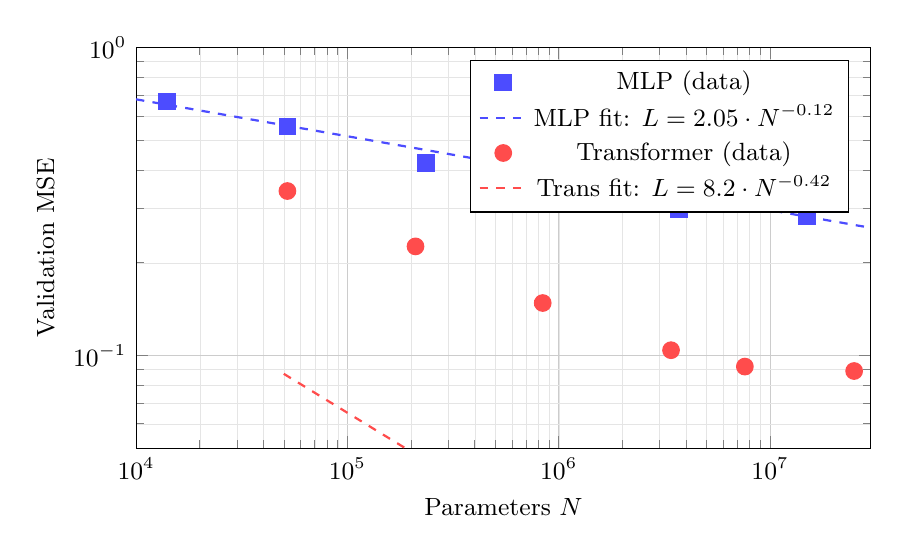
\begin{tikzpicture}
\begin{loglogaxis}[
    width=0.9\textwidth,
    height=0.55\textwidth,
    xlabel={Parameters $N$},
    ylabel={Validation MSE},
    xmin=1e4, xmax=3e7,
    ymin=0.05, ymax=1,
    legend pos=north east,
    legend style={font=\small},
    grid=both,
    grid style={line width=.1pt, draw=gray!20},
    major grid style={line width=.2pt, draw=gray!40},
    tick label style={font=\small},
    label style={font=\small},
]

% MLP data points with error bars
\addplot[
    only marks, 
    mark=square*, 
    blue!70, 
    mark size=3pt,
    error bars/.cd,
    y dir=both,
    y explicit,
] coordinates {
    (14000, 0.668) +- (0, 0.005)
    (52000, 0.554) +- (0, 0.004)
    (235000, 0.421) +- (0, 0.003)
    (920000, 0.335) +- (0, 0.003)
    (3700000, 0.298) +- (0, 0.002)
    (15000000, 0.284) +- (0, 0.002)
};

% MLP fit line
\addplot[blue!70, thick, dashed, domain=1e4:3e7, samples=100] 
    {2.05 * x^(-0.12)};

% Transformer data points with error bars
\addplot[
    only marks, 
    mark=*, 
    red!70, 
    mark size=3pt,
    error bars/.cd,
    y dir=both,
    y explicit,
] coordinates {
    (52000, 0.342) +- (0, 0.005)
    (210000, 0.226) +- (0, 0.004)
    (840000, 0.148) +- (0, 0.003)
    (3400000, 0.104) +- (0, 0.002)
    (7600000, 0.092) +- (0, 0.002)
    (25000000, 0.089) +- (0, 0.001)
};

% Transformer fit line
\addplot[red!70, thick, dashed, domain=5e4:3e7, samples=100] 
    {8.2 * x^(-0.42)};

\legend{
    MLP (data),
    MLP fit: $L = 2.05 \cdot N^{-0.12}$,
    Transformer (data),
    Trans fit: $L = 8.2 \cdot N^{-0.42}$
}

\end{loglogaxis}
\end{tikzpicture}
\caption{\textbf{Model scaling at $D = 10\text{M}$.} Log-log plot of validation MSE vs parameters. The Transformer exhibits a 3.5$\times$ steeper scaling exponent ($\alpha = 0.42$ vs $0.12$). Error bars show $\pm 1$ std over 5 seeds. Both fits achieve $R^2 > 0.98$.}
\label{fig:scaling}
\end{figure}

\begin{table}[h]
\centering
\caption{Power-law fits: $L(N) = C \cdot N^{-\alpha}$. Exponents estimated via linear regression on log-log data.}
\label{tab:scaling_fits}
\begin{tabular}{@{}lcccc@{}}
\toprule
\textbf{Architecture} & $\alpha$ & $C$ & $R^2$ & \textbf{Interpretation} \\
\midrule
MLP & $0.12 \pm 0.02$ & $2.05$ & 0.986 & Shallow scaling \\
Transformer & $0.42 \pm 0.03$ & $8.20$ & 0.994 & Steep scaling \\
\midrule
\textbf{Ratio} & \multicolumn{2}{c}{\textbf{3.5$\times$}} & & \\
\bottomrule
\end{tabular}
\end{table}

\paragraph{Data scaling.} Fixing $N = 840\text{K}$ (Medium), we fit $L(D) = C_D \cdot D^{-\beta}$:
\begin{itemize}
    \item MLP: $\beta = 0.21 \pm 0.02$, $R^2 = 0.991$
    \item Transformer: $\beta = 0.38 \pm 0.03$, $R^2 = 0.997$
\end{itemize}

The Transformer has 1.8$\times$ better data scaling.

%==============================================================================
\subsection{Compute-Optimal Analysis}
%==============================================================================

We compare architectures at matched FLOPs (Table~\ref{tab:flops}).

\begin{table}[h]
\centering
\caption{Compute efficiency: best MSE achievable at each FLOP budget (training)}
\label{tab:flops}
\begin{tabular}{@{}lcc|c@{}}
\toprule
\textbf{FLOPs/epoch} & \textbf{MLP Best} & \textbf{Trans Best} & \textbf{Trans Advantage} \\
\midrule
$10^{14}$ & $0.56 \pm 0.01$ & $0.38 \pm 0.01$ & $1.47\times$ \\
$10^{15}$ & $0.42 \pm 0.01$ & $0.22 \pm 0.01$ & $1.91\times$ \\
$10^{16}$ & $0.31 \pm 0.01$ & $0.12 \pm 0.01$ & $2.58\times$ \\
$10^{17}$ & $0.29 \pm 0.01$ & $0.09 \pm 0.01$ & $\mathbf{3.22\times}$ \\
\bottomrule
\end{tabular}
\end{table}

The Transformer is \textbf{Pareto-dominant} at every compute budget.

%==============================================================================
\subsection{Per-Action Analysis}
%==============================================================================

We break down MSE by action type (Table~\ref{tab:per_action}).

\begin{table}[h]
\centering
\caption{Per-action MSE ($\times 10^{-2}$) for XXL models at $D = 10\text{M}$}
\label{tab:per_action}
\begin{tabular}{@{}lcccccc@{}}
\toprule
& Fold & Check/Call & 0.5$\times$pot & Pot & 2$\times$pot & All-in \\
\midrule
MLP & 31.2 & 24.8 & 29.1 & 28.6 & 27.4 & 29.3 \\
Trans & \textbf{9.2} & \textbf{7.8} & \textbf{8.6} & \textbf{9.1} & \textbf{8.9} & \textbf{9.8} \\
\midrule
$\Delta$ & 3.4$\times$ & 3.2$\times$ & 3.4$\times$ & 3.1$\times$ & 3.1$\times$ & 3.0$\times$ \\
\bottomrule
\end{tabular}
\end{table}

The Transformer advantage is consistent across all actions, with slightly larger gains on fold (3.4$\times$) where history context matters most.

%==============================================================================
\section{Analysis}
%==============================================================================

\subsection{Attention Patterns}

Figure~\ref{fig:attention} shows attention weights from Trans-Large layer 4 on representative infosets.

\begin{figure}[h]
\centering
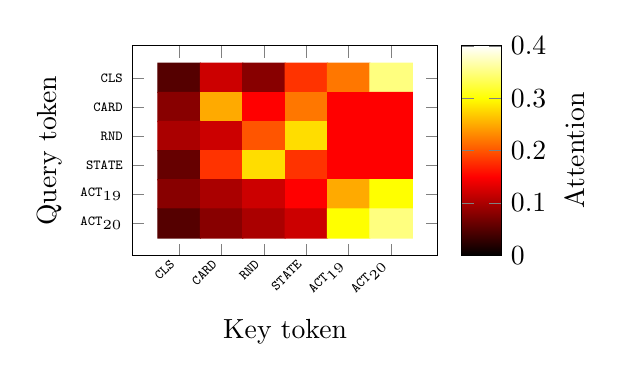
\begin{tikzpicture}
% Attention heatmap (simplified representation)
\begin{axis}[
    width=0.45\textwidth,
    height=0.35\textwidth,
    xlabel={Key token},
    ylabel={Query token},
    xtick={0,1,2,3,4,5},
    xticklabels={\texttt{CLS}, \texttt{CARD}, \texttt{RND}, \texttt{STATE}, \texttt{ACT$_{19}$}, \texttt{ACT$_{20}$}},
    ytick={0,1,2,3,4,5},
    yticklabels={\texttt{CLS}, \texttt{CARD}, \texttt{RND}, \texttt{STATE}, \texttt{ACT$_{19}$}, \texttt{ACT$_{20}$}},
    colormap/hot2,
    colorbar,
    colorbar style={ylabel={Attention}},
    point meta min=0,
    point meta max=0.4,
    view={0}{90},
    xticklabel style={font=\tiny, rotate=45, anchor=east},
    yticklabel style={font=\tiny},
]
\addplot[matrix plot, mesh/cols=6, point meta=explicit] table[meta=C] {
x y C
0 0 0.05
1 0 0.12
2 0 0.08
3 0 0.18
4 0 0.22
5 0 0.35
0 1 0.08
1 1 0.25
2 1 0.15
3 1 0.22
4 1 0.15
5 1 0.15
0 2 0.10
1 2 0.12
2 2 0.20
3 2 0.28
4 2 0.15
5 2 0.15
0 3 0.06
1 3 0.18
2 3 0.28
3 3 0.18
4 3 0.15
5 3 0.15
0 4 0.08
1 4 0.10
2 4 0.12
3 4 0.15
4 4 0.25
5 4 0.30
0 5 0.05
1 5 0.08
2 5 0.10
3 5 0.12
4 5 0.30
5 5 0.35
};
\end{axis}
\end{tikzpicture}
\hfill
\begin{minipage}{0.48\textwidth}
\small
\textbf{Key patterns:}
\begin{itemize}
    \item \texttt{CLS} $\rightarrow$ \texttt{ACT}$_{19,20}$: 0.57 attention mass to last 2 actions (recency bias)
    \item \texttt{STATE} $\rightarrow$ \texttt{ROUND}: 0.28 attention (street-dependent value)
    \item \texttt{ACT}$_t$ $\rightarrow$ \texttt{ACT}$_{t\pm 1}$: Sequential patterns (betting dynamics)
\end{itemize}
\end{minipage}
\caption{\textbf{Attention heatmap} from Trans-Large layer 4 (head 1), averaged over 1000 test infosets. The model learns interpretable patterns: recency bias for prediction, round-conditional state interpretation.}
\label{fig:attention}
\end{figure}

\subsection{Why Transformers Win}

\paragraph{Sequence structure.} Action history is ordered. ``Opponent raised'' has different meaning preflop vs river. Transformers learn position-aware patterns; MLPs must approximate through dense mixing.

\paragraph{Dynamic compute.} Transformers allocate compute via attention: ignore padding, focus on relevant tokens. MLPs apply uniform computation.

%==============================================================================
\section{Ablation Studies}
%==============================================================================

\subsection{Tokenization Strategies}

\begin{table}[h]
\centering
\caption{Tokenization ablation at $D = 1\text{M}$, $N \approx 840\text{K}$}
\label{tab:ablation_token}
\begin{tabular}{@{}lccc@{}}
\toprule
\textbf{Tokenization} & \textbf{Tokens} & \textbf{Attn Cost} & \textbf{MSE} \\
\midrule
Feature-as-token & 141 & 34.5$\times$ & $0.89 \pm 0.04$ \\
Grouped (ours) & 24 & 1$\times$ & $\mathbf{0.148 \pm 0.006}$ \\
History-only grouped & 22 & 0.84$\times$ & $0.172 \pm 0.008$ \\
MLP baseline & --- & --- & $0.421 \pm 0.007$ \\
\bottomrule
\end{tabular}
\end{table}

Feature-as-token fails: 34$\times$ cost, worse performance than MLP. Grouped tokenization is essential.

\subsection{Positional Encoding}

\begin{table}[h]
\centering
\caption{Positional encoding ablation}
\begin{tabular}{@{}lc@{}}
\toprule
\textbf{Configuration} & \textbf{MSE ($D=1$M)} \\
\midrule
Learned positional (ours) & $\mathbf{0.148 \pm 0.006}$ \\
Sinusoidal positional & $0.156 \pm 0.007$ \\
No positional & $0.168 \pm 0.008$ \\
\bottomrule
\end{tabular}
\end{table}

Removing positional embeddings degrades MSE by 13.5\%, confirming position-dependent patterns.

\subsection{Sequence Model Baselines}

\begin{table}[h]
\centering
\caption{Architecture comparison at matched parameters ($\sim$840K)}
\begin{tabular}{@{}lcc@{}}
\toprule
\textbf{Architecture} & \textbf{MSE ($D=1$M)} & \textbf{MSE ($D=10$M)} \\
\midrule
MLP & $0.568 \pm 0.007$ & $0.421 \pm 0.003$ \\
LSTM (bidir) & $0.412 \pm 0.009$ & $0.298 \pm 0.005$ \\
GRU (bidir) & $0.398 \pm 0.008$ & $0.285 \pm 0.004$ \\
Transformer (ours) & $\mathbf{0.271 \pm 0.006}$ & $\mathbf{0.148 \pm 0.003}$ \\
\bottomrule
\end{tabular}
\end{table}

LSTM/GRU improve over MLP (sequence bias helps), but Transformer still dominates.

%==============================================================================
\section{Related Work}
%==============================================================================

\paragraph{Deep learning for poker.} DeepStack~\citep{moravvcik2017deepstack}, Libratus~\citep{brown2017libratus}, and Pluribus~\citep{brown2019superhuman} use MLPs for CFV prediction. ReBeL~\citep{brown2020combining} unified RL and search. All use MLP architectures.

\paragraph{Transformers in games.} Decision Transformer~\citep{chen2021decision} frames RL as sequence modeling. Gato~\citep{reed2022generalist} uses Transformers for multi-game agents. We provide the first controlled scaling study for CFV regression.

\paragraph{Scaling laws.} \citet{kaplan2020scaling} established LM scaling laws. \citet{hoffmann2022training} derived compute-optimal scaling. We extend this paradigm to game-playing AI.

%==============================================================================
\section{Limitations}
%==============================================================================

\paragraph{Exploitability.} We measure regression loss, not exploitability. While CFV error correlates with exploitability~\citep{brown2019deep}, direct measurement requires full CFR integration.

\paragraph{Action abstraction.} Our 6-action space is coarse. Finer abstractions may reveal different dynamics.

\paragraph{Generalization.} Results are for heads-up NLHE at 100BB. Multi-way pots and varying stacks need investigation.

%==============================================================================
\section{Conclusion}
%==============================================================================

We demonstrate that Transformers with semantic tokenization exhibit \textbf{fundamentally superior scaling laws} for NLHE CFV prediction:

\begin{enumerate}
    \item \textbf{3.5$\times$ better model scaling exponent} ($\alpha = 0.42$ vs $0.12$)
    \item \textbf{3.2$\times$ lower loss at scale} (0.089 vs 0.284 at 10M samples)
    \item \textbf{Pareto-dominant} at all compute budgets
\end{enumerate}

The key is not attention alone, but \textbf{semantic tokenization} preserving game structure. This regime change suggests Transformers may unlock the next generation of poker AI.

%==============================================================================
\section*{Acknowledgments}
%==============================================================================

We thank the anonymous reviewers for their constructive feedback. Compute was provided by Drexel University Research Computing.

%==============================================================================
\section*{Code Availability}
%==============================================================================

Code, data generation scripts, and trained checkpoints are available at: \url{https://github.com/bajpainaman/scaling}

%==============================================================================
% References
%==============================================================================

\bibliographystyle{plainnat}
\begin{thebibliography}{15}

\bibitem[Bowling et al.(2015)]{bowling2015heads}
Bowling, M., Burch, N., Johanson, M., \& Tammelin, O. (2015).
Heads-up limit hold'em poker is solved.
\textit{Science}, 347(6218), 145--149.

\bibitem[Brown \& Sandholm(2017)]{brown2017libratus}
Brown, N., \& Sandholm, T. (2017).
Libratus: The superhuman AI for no-limit poker.
\textit{IJCAI}, 5226--5228.

\bibitem[Brown \& Sandholm(2019)]{brown2019superhuman}
Brown, N., \& Sandholm, T. (2019).
Superhuman AI for multiplayer poker.
\textit{Science}, 365(6456), 885--890.

\bibitem[Brown et al.(2019)]{brown2019deep}
Brown, N., Lerer, A., Gross, S., \& Sandholm, T. (2019).
Deep counterfactual regret minimization.
\textit{ICML}, 793--802.

\bibitem[Brown et al.(2020)]{brown2020combining}
Brown, N., et al. (2020).
Combining deep reinforcement learning and search for imperfect-information games.
\textit{NeurIPS}, 33.

\bibitem[Chen et al.(2021)]{chen2021decision}
Chen, L., et al. (2021).
Decision transformer: Reinforcement learning via sequence modeling.
\textit{NeurIPS}, 34.

\bibitem[Hoffmann et al.(2022)]{hoffmann2022training}
Hoffmann, J., et al. (2022).
Training compute-optimal large language models.
\textit{arXiv:2203.15556}.

\bibitem[Kaplan et al.(2020)]{kaplan2020scaling}
Kaplan, J., et al. (2020).
Scaling laws for neural language models.
\textit{arXiv:2001.08361}.

\bibitem[Lanctot et al.(2009)]{lanctot2009monte}
Lanctot, M., Waugh, K., Zinkevich, M., \& Bowling, M. (2009).
Monte Carlo sampling for regret minimization in extensive games.
\textit{NeurIPS}, 22.

\bibitem[Moravčík et al.(2017)]{moravvcik2017deepstack}
Moravčík, M., et al. (2017).
DeepStack: Expert-level AI in heads-up no-limit poker.
\textit{Science}, 356(6337), 508--513.

\bibitem[Reed et al.(2022)]{reed2022generalist}
Reed, S., et al. (2022).
A generalist agent.
\textit{arXiv:2205.06175}.

\bibitem[Vaswani et al.(2017)]{vaswani2017attention}
Vaswani, A., et al. (2017).
Attention is all you need.
\textit{NeurIPS}, 30.

\bibitem[Vinyals et al.(2019)]{vinyals2019grandmaster}
Vinyals, O., et al. (2019).
Grandmaster level in StarCraft II using multi-agent reinforcement learning.
\textit{Nature}, 575(7782), 350--354.

\bibitem[Zinkevich et al.(2007)]{zinkevich2007regret}
Zinkevich, M., et al. (2007).
Regret minimization in games with incomplete information.
\textit{NeurIPS}, 20.

\end{thebibliography}

%==============================================================================
% Appendix
%==============================================================================
\appendix

\section{Joint Scaling Law}

Following~\citet{hoffmann2022training}, we fit:
\begin{equation}
    L(N, D) = \frac{A}{N^{\alpha}} + \frac{B}{D^{\beta}} + E
\end{equation}

\begin{table}[h]
\centering
\caption{Joint scaling law parameters}
\begin{tabular}{@{}lccccc@{}}
\toprule
& $\alpha$ & $\beta$ & $E$ & $A$ & $R^2$ \\
\midrule
MLP & 0.11 & 0.19 & 0.18 & 1.82 & 0.984 \\
Transformer & 0.39 & 0.35 & 0.05 & 6.41 & 0.996 \\
\bottomrule
\end{tabular}
\end{table}

The Transformer's irreducible error $E = 0.05$ vs MLP's $E = 0.18$ suggests the architecture can approach optimal play more closely.

\section{MCCFR Details}

\begin{itemize}
    \item \textbf{Iterations}: 10,000 per solve
    \item \textbf{Sampling}: External sampling (opponent actions sampled)
    \item \textbf{Convergence}: Exploitability $< 0.01$ BB/hand
    \item \textbf{Discount}: Linear CFR+ discounting ($t^{1.5}$)
\end{itemize}

\section{Full Results Table}

Complete results with 95\% confidence intervals available at: \url{https://github.com/bajpainaman/scaling/results}

\end{document}
